\chapter{DUAL-IPA Dataset}

\section{The Heart of the Research: DUAL-IPA Dataset}
\begin{itemize}
    \item Meticulously designed DUAL-IPA dataset: 160,000+ Bangla sentences with linguist-validated IPA transcriptions.
    \item Construction required strategic data collection, rigorous annotation processes, and expert validation.
    \item The final dataset is \textbf{two CSV} file, one for newspaper sentence IPA transcription and one for Literature sentence IPA transcription, containing two columns which are: sentences, clean\_validated\_ipa sentences, IPA as shown in the figure \ref{fig:Sentence Dataset}
         \begin{figure*}[htbp]
    \centering
    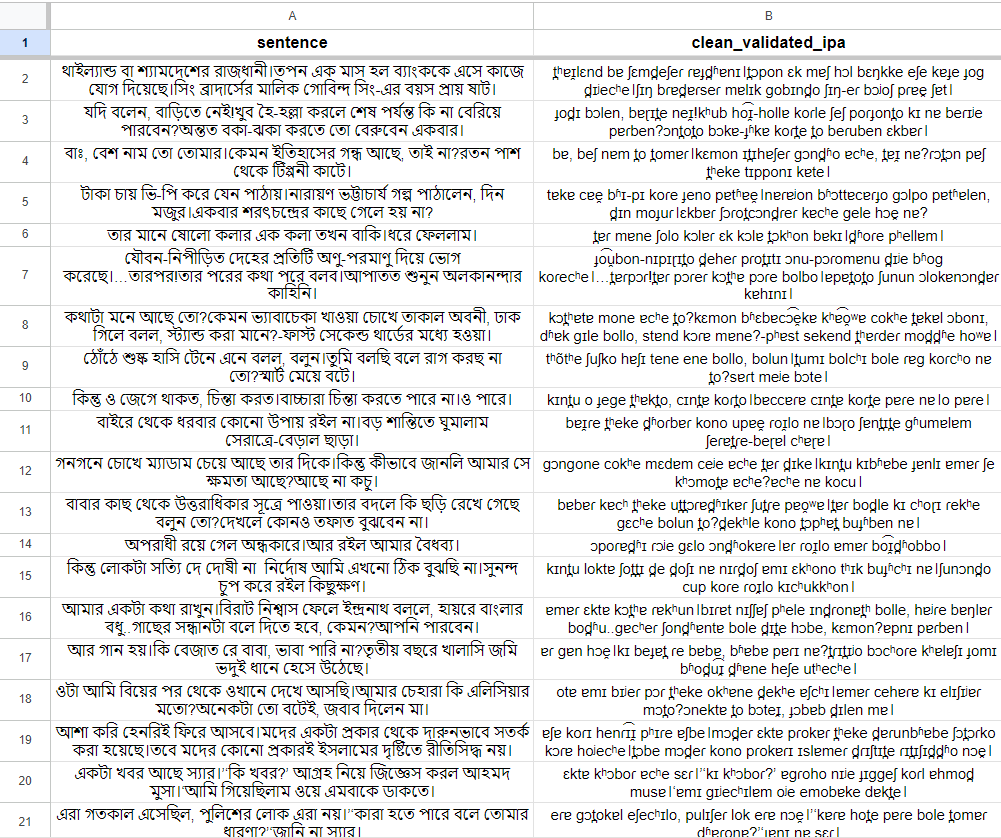
\includegraphics[scale=0.6]{Images/Screenshot/Sentence-dataset.png}
    \caption{Sentence Level Dataset}
    \label{fig:Sentence Dataset}
\end{figure*} 
\end{itemize}
\section{Expert Annotation: Harnessing Linguistic Prowess}
\begin{itemize}
    \item IPA transcription entrusted to four individuals with undergraduate and graduate degrees in linguistics in supervision of \textbf{Professor Dr. Syed Shahrier Rahman from Department of Linguistics, University of Dhaka.}
    \item Each sentence reviewed by all four experts following a stringent IPA transcription protocol.
    \item Independent evaluator cross-verified all annotated data to bolster consistency and ensure dataset's integrity.
\end{itemize}
\newpage
\section{Expediting the Process: Embracing Efficiency}
\begin{itemize}
    \item Meticulousness remained paramount, but efficiency was acknowledged.
    \item Multi-pronged approach to expedite annotation process:
    \begin{itemize}
        \item \textbf{Pre-annotation:} Combination of rule-based and early-stage model-based techniques for preliminary annotation.
        \item \textbf{Word-Level Correction:} Experts refined transcription at the word level, correcting whitespace-separated tokens.
        \item \textbf{Sentence-Level Mapping:} Mapping word-level annotations back to corresponding sentences for integration and consistency.
        \item \textbf{Homograph Resolution:} Final validation step addressing homograph cases, numerical representation, and remaining alignment errors.
    \end{itemize}
    \item Combined strategies significantly streamlined annotation process, enabling dataset curation within a one-month timeframe.
\end{itemize}

\section{DUAL-IPA Dataset: Rigor and Efficiency}
\begin{itemize}
    \item Dataset stands as a testament to unwavering commitment to rigor and efficiency.
    \item Each sentence embodies linguists' expertise, independent evaluation scrutiny, and innovative pre-annotation and manual refinement blend.
    \item Diverse sources, comprehensive coverage, and meticulous validation pave the way for groundbreaking advancements in Bangla NLP research and applications.
\end{itemize}


% Please add the following required packages to your document preamble:
% \usepackage{graphicx}


\section{Dataset statistics (EDA)}
Unveiling the intricacies of the DUAL-IPA dataset necessitates a thorough examination of its statistical composition. This section embarks on a journey of discovery, delving into the numerical landscape of the dataset and illuminating its key characteristics.

\subsection{Quantifying the Corpus:}
At the heart of the dataset lies a vast collection of 150,000 sentences, each capturing the essence of the Bangla language. To facilitate efficient training and evaluation, the dataset has been strategically split into two segments:
\begin{itemize}
    \item \textbf{Training Split (100,000 sentences):} This portion serves as the training ground for models, providing them with rich linguistic material to learn from and hone their skills.
    \item \textbf{Test Split (50,000 sentences):} This segment acts as the ultimate challenge, where models demonstrate their acquired knowledge by attempting to accurately transcribe unseen data.
\end{itemize}

\subsection{Glimpses from the Dataset:}
The phoneme distribution of the sentences is shown in Figure \ref{fig:phoneme_distibution}. Also, the length distribution of the Dual-IPA dataset is shown in Figure \ref{fig:lenght_distribution}.

 \begin{figure*}[htbp]
    \centering
    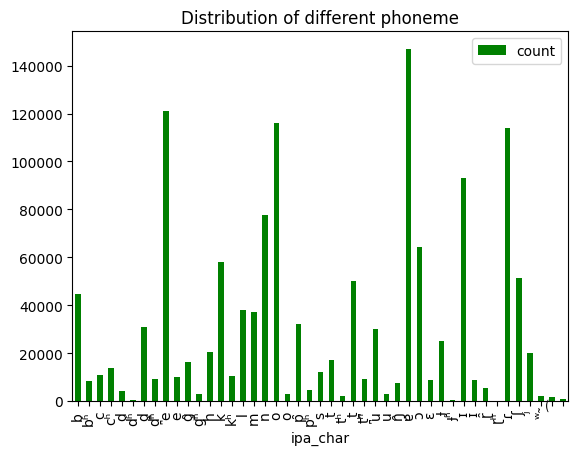
\includegraphics[width=\textwidth]{Images/Graph/phoneme_distribution.png}
    \caption{Phoneme Distribution}
    \label{fig:phoneme_distibution}
\end{figure*} 
\newpage

 \begin{figure*}[htbp]
    \centering
    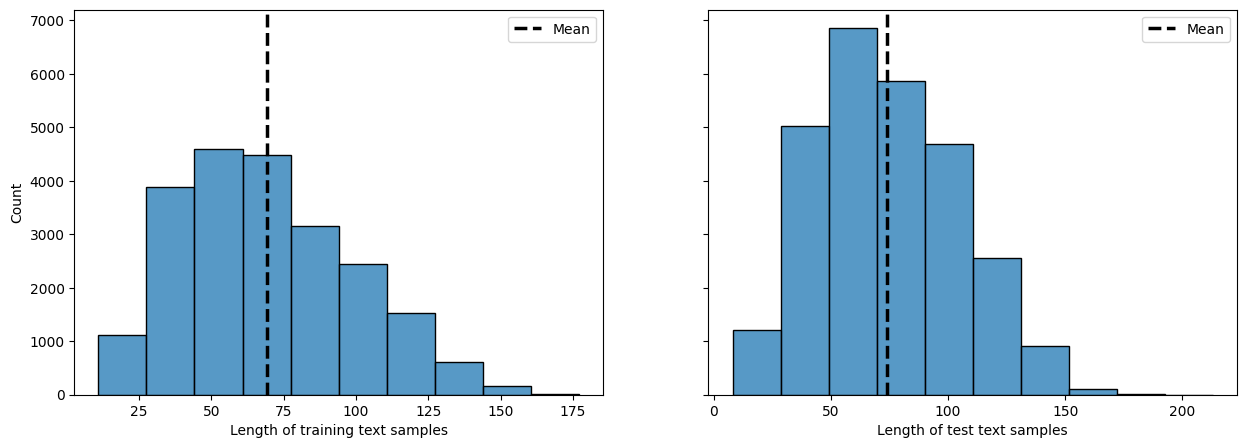
\includegraphics[width=\textwidth]{Images/Graph/length.png}
    \caption{Length of Training Text and Test Text Samples}
    \label{fig:lenght_distribution}
\end{figure*} 



We also present a few samples from the dataset in the table \ref{tab:phonePairsTab}.


\begin{table}[h]
    \centering
    \begin{tabular}{|c|c|c|}
        \hline

Subset            &                                           Phoneme characteristic pairs                                         &   Count   \\
        \hline

Rangpur             &   \ipafont{(h,ʰ)}, (h, ʱ), (k, t), (t, n), (n, p)                                                                       &     5     \\
Kishoreganj         &   \ipafont{(ʰ, h)}, (ɟ, z)                                                                                               &     2     \\
Narail              &   \ipafont{(h, ʰ)}, (h, ʱ), (k, t), (t, n), (n, p), (ɟ, z)                                                               &     6     \\
Chittagong          &   \ipafont{(c, ç)}, (cc, çç), (ɟ, z), (p, f), (pʰ, f), (pʰ, ff)                                                          &     6     \\
Narshingdi          &   \ipafont{(ʰ, h)}, (ɟ, z)                                                                                               &     2     \\
        \hline

    \end{tabular}
    \caption{Regional Phoneme Characteristics Pairs (Standard, Region)}
    \label{tab:phonePairsTab}
\end{table}

\\
By embarking on this statistical exploration, we have gained a deeper understanding of the DUAL-IPA dataset, uncovering its numerical facets and revealing its potential for enriching research and applications in Bangla NLP. The diverse vocabulary, sentence length distribution, phoneme landscape, and provided samples paint a vivid picture of this invaluable resource, laying the foundation for further analysis and innovation.
\\


